\newpage
%%%%%%%%%%%%%%%%%%%%%%%%%%%%%%%%%%%%%%%%%%%%%%%%%%%%%%%%%%%%%%%%
%%%%%%%%%%%%%%%%%%%%%%%%%%%%%%%%%%%%%%%%%%%%%%%%%%%%%%%%%%%%%%%%
%%%%%%%%%%%%%%%%%%%%%%%%%% Enunciado %%%%%%%%%%%%%%%%%%%%%%%%%%%

\begin{myblock}
\phantomsection\addcontentsline{toc}{section}{Parte A | RNN}
\section*{Parte A | RNN}

    Entrena los modelos con las canciuones y con las arquitecturas RNN/LSTM/GRU. A nivel
    caracter y a nivel palabra.

\end{myblock}

%%%%%%%%%%%%%%%%%%%%%%%%%%%%%%%%%%%%%%%%%%%%%%%%%%%%%%%%%%%%%%%%
%%%%%%%%%%%%%%%%%%%%%%%%%%%%%%%%%%%%%%%%%%%%%%%%%%%%%%%%%%%%%%%%

%\begin{figure}[h!]
%   \centering
%   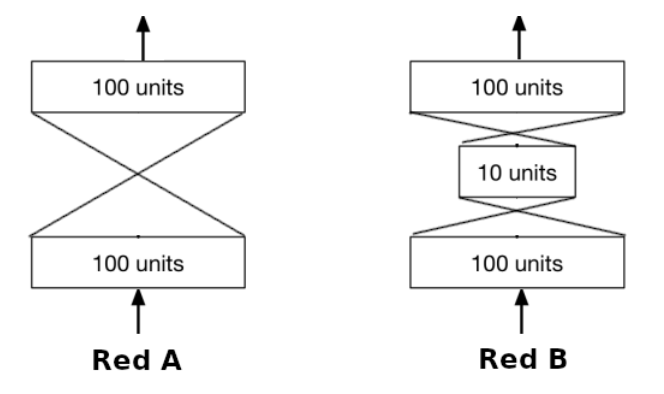
\includegraphics[width=0.8\linewidth]{Images/redA-redB.png}
%   \caption{Esquema de dos redes neuronales.}
%   \label{fig:redA_redB}
%\end{figure}


%%%%%%%%%%%%%%%%%%%%%%%%%%%%%%%%%%%%%%%%%%%%%%%%%%%%%%%%%%%%%%%%
%%%%%%%%%%%%%%%%%%%%%%%%%%%%%%%%%%%%%%%%%%%%%%%%%%%%%%%%%%%%%%%%

Los modelos de lenguaje (LM por sus siglas en inglés), buscan asignar probabilidades 
a secuecnias de palabras o caracteres y, en particular, estimar la probabilidad del 
siguiente token dado el contexto previo. Durante décadas, esto se abordó con n-gramas;
la métrica canónica es la perplejidad (PPL), la cual se definió como el exponencial de
la entropía cruzada priomedio, o de manera equivalente, es la inversa de la probabilidad
media del corpus. Minimizar la perplejidad es maximizar la probabilidad de los datos, y 
cuanto menor es la PPL, mejor el modelo en términos de sorpresa promedio por token. 

En ese sentido, las Redes Neuronales Recurrentes (RNN), introdujeron una forma distinta de trata el tiempo. Es decir, las RNN comparten pesos a lo largo de la secuencia y actualizan un estado oculto que "transporta" la información entre pasos, permitiendo modelar dependencias más largas que las que capturan n-gramas. Este paradigma dio paso a variantes con compuertas, que veremos más adelante, como lo son las LSTM y GRU. Fueron la piedra de inicio que también dio el primer paso para llegar a lo que ahora conocemos como Transformers y que son la base para los LLM. 

Aún así, las RNN y sus variantes siguen siendo fundamentales como baselines y por su valor didáctico, pues son la puerta de incio para el aprendizaje por secuencias y el Procesamiento de Lenguaje Natural con modelos de Redes Neuronales. 

\subsection{Formulación probabilística de los Modelos de Lenguaje (ML)}

Sea $\omega_1;T$ una secuencia. Un LM autoregresivo factoriza la probabilidad conjunta como:

\[
    p(\omega_{1;T}) = \prod_{t=1}^T p(\omega_t | \omega_{<t})
\]

Esta descomposición habilita el aprendizaje autosupervisado, i.e. donde cada paso temporal proporciona su propio "objetivo", de tal modo que $\omega_t$ se predice a partir de $\omega_{<t}$. El entrenamiento minimiza la entropía cruzada promedio (NLL), y la perplejidad se define como $\text{PPL} = \exp(\text{CE Promedio})$. 

Un procedimiento práctico asociado es el \textit{teacher forcing}: durante el entrenamiento, el modelo recibe como entrada el token veraddero del paso anterior y aprende a predecir el siguiente. 

\subsection{Arquitectura de las RNN}

En una RNN "simple", cada entrada $x_t$ (el embedding del token en $t$), actualiza el estado oculto $h_t$ con pesos compartidos.

En esta formulación, los parámetros de la red se organizan en tres matrices fundamentales que gobiernan el flujo de información:

\begin{itemize}
    \item $W_{xh}$ (a menudo denotada $U$) transforma la representación de entrada $x_t$ hacia el espacio del estado oculto.
    \item $W_{hh}$ (denotada en algunos textos como $W$) es la matriz recurrente que proyecta el estado oculto previo $h_{t-1}$ y permite transportar la información a lo largo de la secuencia.
    \item $W_{ho}$ (o $V$) mapea el estado oculto actual $h_t$ hacia el espacio de salida, produciendo los logits sobre el vocabulario.  
\end{itemize}

Estas matrices son compartidas en todos los pasos temporales, lo cual constituye la esencia de la recurrencia: el modelo reutiliza los mismos parámetros para procesar cualquier posición de la secuencia, logrando generalizar más allá de la ventana fija de los modelos n-grama.

\[
h_t = \phi(W_{xh}x_t + W_{hh} h_{t-1} + b_h) \;\;\;\;\;\;\;\;\;\; o_t = W_{h0}h_t + b_{o} \;\;\;\;\;\;\;\;\;\; \hat{y}_t = \text{Softmax}(o_t)
\]

Aquí, $\hat{y}_t$ es la distribución sobre sobre el vocabulario para le próximo token. Esta arquitectura se desenrolla en el tiempo para visualizar el flujo de información y de gradientes a lo largo de las secuencias. 

Acorde con Dan Jurafsky en el libro 'Speech and Language Processing', las  capas ocultas de los pasos anteriores funcionan a manera de memoria, o de contexto. Se trata de una especie de sistema que procesa la información para posteriormente tomar la decisión más adelante en el entrenamiento. Además, los pesos y el flujo tras cada capa lleva arrastrando todo el contexto anterior, no hay un límite en cuanto a la "cantidad" de contexto que se puede llevar cargando. Al menos en el modelo base de RNN. 

El entrenamiento de una RNN es un poco distinto al de un MLP tradicional. El backpropagation de las recurrentes sucede en dos pasos: primero se realiza inferencia hacia adelante, calculando tanto $h_t$ como $y_t$, y se acumula la pérdida tras cada avance a lo largo del tiempo, siempre guardando los valores de las capas ocultas tras cada paso para su uso posterior. Después, el segundo paso, es el procesamiento de la secuencia en reversa, donde se calculan lo sgradientes requeridois, logrando el cómputo y guardado dle término de error para usarlo en la capa oculta para cada paso hacia atrás. Jurafsky menciona que este proceso es llamado: "backpropagation a través del tiempo". 

Los modelos de lenguaje de las RNN procesan las secuencias de entrada una palabra a la vez. Es decir, lo que se intenta es predecir la palabra que sigue a partir de la palabra actual inmediata y el estado oculto anterior. Es por ello que las RNN se diferencían claramente de los n-gramas, pues estos tienen contexto limitado, y a diferencia del contexto fijo de modelos clásicos, son un sistema que no tiene límite de contexto en cuanto a todo lo que puede arrastrar desde sus secuencias de entrada iniciales. 


\subsection{Arquitectura Utilizada e Hiperparámetros}

Finalmente, para establecer una línea base de comparación, se implementó un modelo utilizando una Red Neuronal Recurrente simple (RNN). Aunque es susceptible al problema del desvanecimiento del gradiente en secuencias muy largas, su arquitectura más sencilla sirve como un punto de referencia fundamental para evaluar la ganancia en rendimiento obtenida con las arquitecturas más complejas de compuertas como GRU y LSTM.

Al igual que con los modelos anteriores, la configuración se mantuvo consistente para los entrenamientos a nivel de carácter y palabra.

\subsubsection{Estructura del Modelo}

La arquitectura del modelo RNN se diseñó con una mayor dimensionalidad en su estado oculto para compensar la simplicidad relativa de su unidad recurrente. La estructura fue la siguiente:

\begin{enumerate}
    \item \textbf{Capa de Embedding:} Una capa inicial para convertir los tokens de entrada en vectores densos. Se asumió una dimensión de embedding de 128 para mantener la consistencia con las otras arquitecturas.

    \item \textbf{Capas RNN Apiladas:} El núcleo del modelo consiste en 4 capas de RNN simple apiladas. Cada capa fue configurada con una dimensión de estado oculto (\texttt{hidden\_dim}) de 512 unidades, un tamaño mayor para aumentar la capacidad de representación del modelo.

    \item \textbf{Capa de Regularización (Dropout):} Se aplicó una tasa de \texttt{Dropout} del 30\% (0.3) entre las capas recurrentes para controlar el sobreajuste.

    \item \textbf{Capa de Salida (Clasificador):} Una capa lineal final proyecta la salida de la última capa RNN al tamaño del vocabulario, utilizando una función de activación \texttt{Softmax} para la predicción del siguiente token.
\end{enumerate}

\subsubsection{Hiperparámetros de Entrenamiento}

Los hiperparámetros utilizados para el entrenamiento del modelo RNN se detallan en la Tabla \ref{tab:rnn_hyperparams}. Se optó por un número menor de épocas de entrenamiento en comparación con los otros modelos, debido a la mayor rapidez con la que las RNN simples tienden a converger o a sobreajustar.

\begin{table}[h!]
    \centering
    \caption{Resumen de hiperparámetros de entrenamiento para el modelo RNN simple.}
    \label{tab:rnn_hyperparams}
    \begin{tabular}{l|l}
        \hline
        \textbf{Hiperparámetro} & \textbf{Valor Utilizado} \\ \hline
        Optimizador & \texttt{Adam} \\
        Tasa de Aprendizaje (Learning Rate) & \texttt{5e-4 (0.0005)} \\
        Función de Pérdida & \texttt{Cross-Entropy Loss} \\
        Tamaño del Lote (Batch Size) & \texttt{32} \\
        Épocas de Entrenamiento & \texttt{12} \\
        Semilla Aleatoria (Seed) & \texttt{42} \\ \hline
    \end{tabular}
\end{table}

\subsection{Resultados}

\begin{lstlisting}[
    style=mystyle,
    caption={Output crudo del modelo generativo a nivel de carácter.},
    label={lst:output-char-level}
]
I <UNK> <UNK> <UNK> <UNK> <UNK> <UNK> <UNK>  p l a n n e d  T h e r e ' s  s o m e o n e  e l s e ' s  d r e a m s ?  ( E l s e ' s  d r e a m s ?  ( E l s e ' s  d r e a m s ?  W h i n e  a l l ,  k n o w  T h a t  t h e y  t o l d  m e  I  w a s  g o n e  B u t  I ' l l  n e v e r  b e t t e r  o f f  m y  h e a d )  L e a r n i n g  d a r d y  s o  h a p p e n ?  W h a t  h a v e  a  c h a i n ' s  i c s  i n  y o u r  p a c e s ,  B l u r r y f a c e s  o f  f e e l i n '  s p u l l  s t i l l  a r e  s i t c i n g  G o t  t o  t h i s  t i m e  I ' l l  s i t  h e r e  ' t i l  I  f i n d  t h e  p r o b l e m  N o ,  I  m o v e  s l o w  I  w a n t  t o  s t o p  t i m e  I ' l l  s i t  h e r e  ' t i l  I  f i n d  t h e  p r o b l e m  N o ,  I
\end{lstlisting}

\clearpage

\begin{lstlisting}[
    style=mystyle,
    caption={Output crudo del modelo generativo a nivel de palabra.},
    label={lst:output-word-level}
]
<UNK> like my soul but not my mind is n't helping , saturday when it 's for the night 's decor it reveals what we dream of i have to know and i 'm a lot , right in one piece now i asked me , " son , when i grow old will you buy me a house of gold ? and when your father turns to stone will you take care of me ? " i will make you queen of everything you see i 'll put you on the map i 'm driving ' our thumbs for ammunition i was born a choker nobody 's comin ' for me comin ' for me from it 's decidin fine that part they form a lot with it 's real 'cause i told you you are out of my mind heard you say ( " today " 'cause the heat , place chances straight ever smell , you know that kills 's coming and welcome to the style you have n't seen in a while it 's lavish ( feeling gourmet ) welcome to the new way of living it 's just the beginning of lavish from the floor ( we 're broken too , yeah )
\end{lstlisting}

\subsubsection*{PPL por época}

\begin{figure}[h!] 
    \centering
    \caption{Comparación de la perplejidad (PPL) por época para los modelos RNN.}
    \label{fig:rnn_ppl_comparacion}

    \begin{subfigure}[b]{0.48\textwidth}
        \centering
        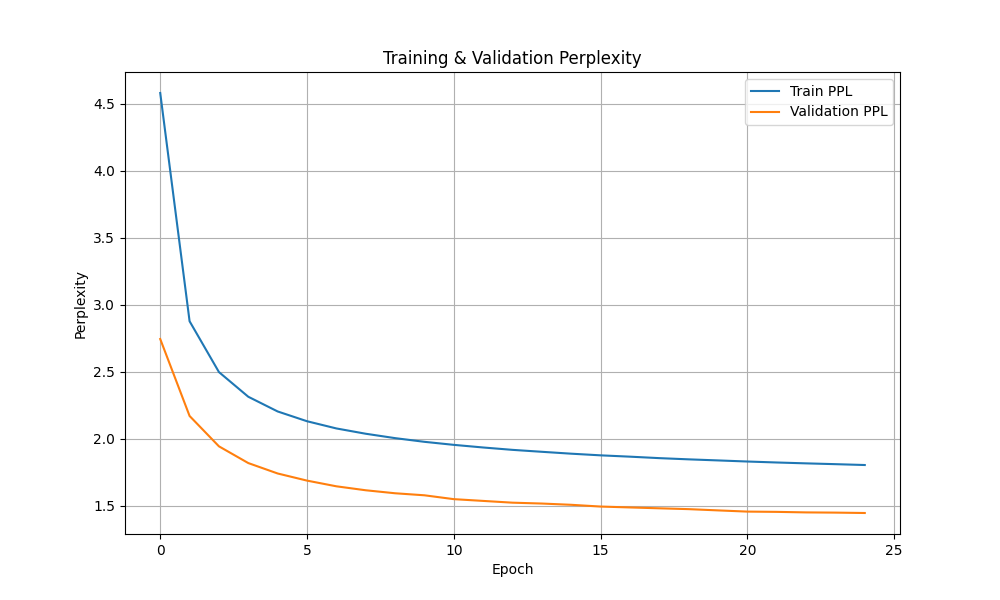
\includegraphics[width=\textwidth]{Images/rnn_training_history_c.png}
        \caption{Modelo a Nivel de Carácter.}
        \label{fig:rnn_ppl_char}
    \end{subfigure}
    \hfill % Este comando crea un espacio elástico entre las dos figuras
    \begin{subfigure}[b]{0.48\textwidth}
        \centering
        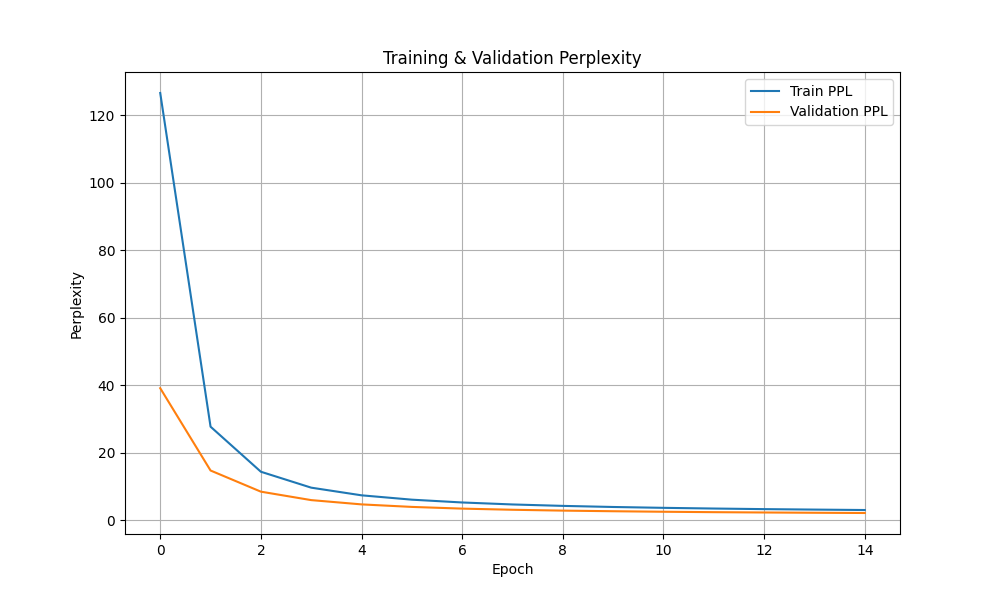
\includegraphics[width=\textwidth]{Images/rnn_training_history_w.png}
        \caption{Modelo a Nivel de Palabra.}
        \label{fig:rnn_ppl_word}
    \end{subfigure}
\end{figure}

\subsection{Conclusiones}

En primer lugar, podemos mencionar que los resultados de PPL muestran una clara diferencia
entre los modelos a nivel de carácter y a nivel de palabra. El modelo char-level alcanzó valores
de validación cercanos a 1.44 tras 25 épocas, indicando una buena capacidad de predicción local, 
aunque con salidas generativas afectadas por la presencia de múltiples \texttt{<UNK>}. Esto 
es muy probablemente debido a la forma en que se introdujo el promt inicial, pues no se tokenizó
a nivel carácter por carácter, lo que impidió al modleo explotar de manera correcta su estado
inicial. A pesar de ello, la disminución progresiva y estable de la PPL parece sugerir que el 
modelo aprendió bien acerca de regularidades ortográficas y patrones. 

Por otra parte, el modelo word-level presentó inicialmente una perplejidad muy alta, de hecho, 
superior a 100, pero convergió rápido hasta valores cercanos a 2.08 en el conjunto de validación.
Esto refleja que, aun con un corpus de tamaño limitado, las representaciones distribuidas de palabras
permiten capturar dependencias más semánticas y temáticas. Esta muestra refleja que a nivel palabras
hay una mejor coherencia y frases reconocibles dentro edl estilo lírico de Twenty One Pilots, 
aunque no sin redundancias y repeticiones frecuentes. 

La métrica de novelty confirma dichas tendencias. Los modelos LSTM y GRU (que veremos más adelante),
a nivel palabra, alcanzaron los valores más altos de novedad trigramal con $\sim 0.92$, mientras
que la RNN simple mostró mayor tendencia a memorizar, con un valor de 0.22 en trigramas. Esto implica
que las arquitecturas con puertas de memoria favorecen una mejor capacidad de recombinar fregmentos
de texto en lugar de limitarse a repetir secuencias vistas durante el enternamiento. 

En cuanto a la calidad cualitativa de las letras generadas, los outputs a nivel carácter tienden 
a generar secuencias ruidosas y poco interpretables, mientras que a nivel palabra están mejor
estructurados, con una mejor gramática, mejores referencias líricas y elementos estilísticos
asociado a la banda, aunque noto que esto provoca la repetición de frases que vuelve al modelo
poco creativo. Esto es reflejo de la limitaciones por el tamaño del corpus, provocando poca 
diveridad y la generacón de clichés.

Adelantandonos un poco a lo siguientes modelo, la RNN presentan mayor tendencia a memorizar 
y a repetir. Asimismo, la generación a nivel palabra logra capturar mejor el estilo y temática
del corpus. Ojalá tuvieramos mil canciones de Twenty One Pilots mas, para poder entrenar un LM
más solido. 



\clearpage










